\subsection{$D$ and $B$ mesons}
A high statistics sample of pPb collisions will be extremely useful 
to test heavy-flavour production over a wide transverse momentum range.
At low $\rm p_{T}$, the study of the nuclear modification factors of 
D and B mesons allows to test the relevance of cold nuclear matter 
effects in the heavy flavour sector~\cite{Eskola:2009uj,deFlorian:2003qf,Frankfurt:2011cs}. 
Gluon saturation processes are expected to reduce the production 
cross sections of D mesons of about 10-20$\%$ at about 2-3 GeV/c.  
In the B sector, a smaller modification is expected as a consequence 
of the large $x$ range that we investigate with this measurement.
A precise measurement of the D and B nuclear modification factors 
in pPb collisions at low $\rm p_{T}$ is therefore needed to experimentally 
validate the theoretical expectations. In Fig~\ref{fig:measurementB}, 
the current measurement performed at 5.02 TeV with $\rm L_{int}$=34.8/nb 
is presented~\cite{PhysRevLett.116.032301}. The current statistical 
and systematic uncertanties do not allow to appreciate any significant 
deviation from unity. In Fig~\ref{fig:Bextrapolated}, the result expected 
at 8 TeV considering an integrated luminosity of 100/nb is presented. 
In order to have the possibility to measure the B production down to 
low $\rm p_{T}$ with the needed accuracy (~5-10$\%$), 
the largest luminosity available is therefore strictly necessary.  
A larger sample of 8 TeV pPb data would also be beneficial for heavy 
flavor studies at high $\rm p_{T}$.  In Fig~\ref{fig:plotsDBpredictions}, 
the FONLL predictions for D (left) and B (right) cross sections are shown. 
An increase of the heavy-flavour cross section of about 2 is
expected at $\rm p_{T}~$100 GeV/c as a consequence of the larger 
center-of-mass value. 

\begin{figure}[h]
\begin{center}
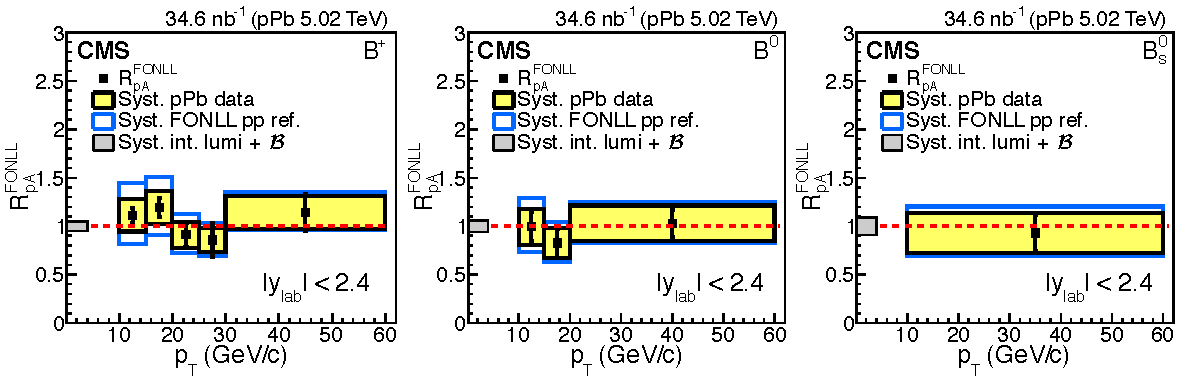
\includegraphics[width= 0.95\textwidth]{figures/nuclearmodification.pdf}
\caption{Nuclear modification factor in pPb collisions at \rootsNN\ = 5.02 TeV 
obtained with L$_{\rm int}$ = 35 nb$^{-1}$~\cite{PhysRevLett.116.032301}.}
\label{fig:measurementB}
\end{center}
\end{figure}

\begin{figure}[h]
\begin{center}
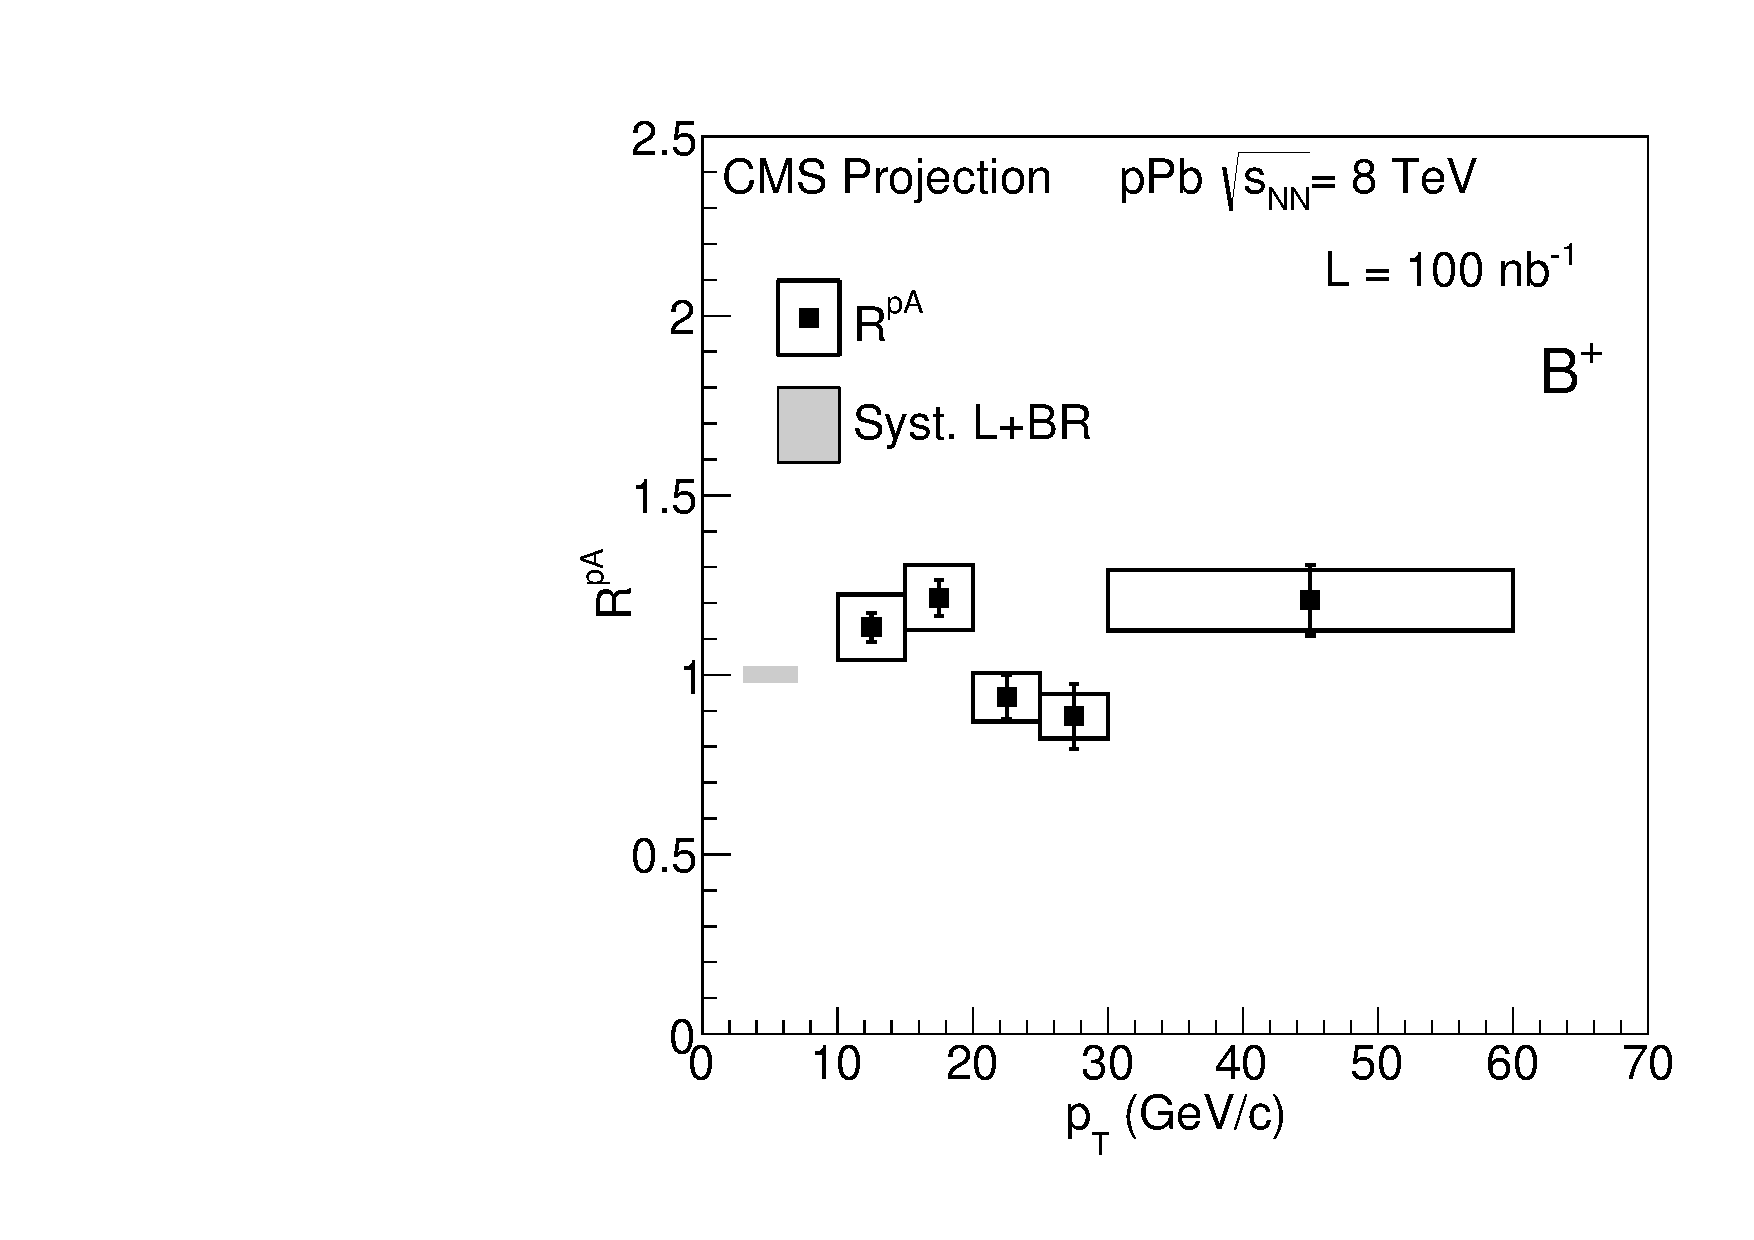
\includegraphics[width= 0.55\textwidth]{figures/canvasrpabplus}
\caption{Projected $\rm B^{+}$ meson $\rm R_{pPb}$ estimated for pPb collisions at \rootsNN\ = 8.16 TeV 
with L$_{\rm int}$ = 100 nb$^{-1}$ based on 2011 pPb measurement.}
\label{fig:Bextrapolated}
\end{center}
\end{figure}

\begin{figure}[h]
\begin{center}
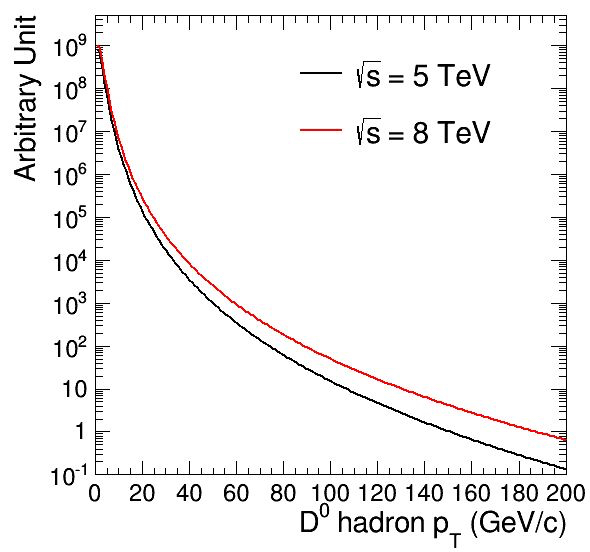
\includegraphics[width= 0.45\textwidth]{figures/D-Sigma.jpg}
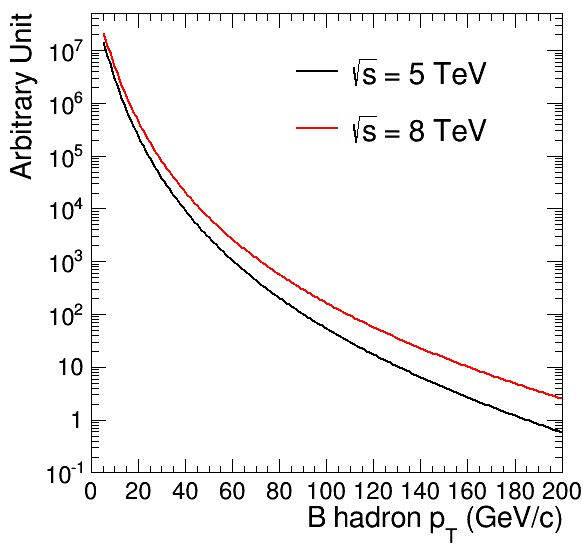
\includegraphics[width= 0.45\textwidth]{figures/B-Sigma.jpg}
\caption{FONLL predictions for $D$ (left) and $B$ (right) meson production at \rootsNN\ = 8.16 and 5.02 TeV
 as a function of \pt\ ~\cite{FONLLcharmbottomPP1}.}
\label{fig:plotsDBpredictions}
\end{center}
\end{figure}
